\subsection{Global Interconnect Networks}

Ever since the first international mobile communication standard \gls{gls:2g}/GSM, Mobile Network Operators around the world exchange signaling and user data via the global \gls{ipx} network.
Designed to be a private channel for communication amongst \glspl{mno} only, the way in which it is used today, and the plethora of different agents connected to it --many of them not network operators-- renders it a network that is not any more trustworthy than the public internet.
Coupled with weaknesses in the established network protocols as previously summarized in section \ref{sec:related}, the interconnect interface is cause for major security and fraud concerns for any mobile operator.

One of the reasons why this well-known problem still persists several years after the publication of possible exploits is the role that operators of \gls{ipx} peering platforms play in inter-\gls{plmn} signaling, which goes well beyond that of pure connectivity providers.
Many \glspl{mno} depend on them for supplementary services that require to access or even modify the contents of the signaling traffic.
These services include, for example, normalization of the protocol syntax, replacement of attributes to alleviate technical incompatibilities, and business intelligence offerings.
Note that for the communication partners on either side it is intransparent which routing path messages take on the interconnect network.
A single \gls{plmn} can simultaneously be connected to multiple \gls{ipx} providers, which in turn may or may not connect directly to each other.
\gls{3gpp} assumes a model in which there is at least one or more \gls{ipx} provider in any given routing path (see \cite{3gpp.33.501}, 130):

\begin{enumerate}[label=--]
    \item Both \glspl{plmn} are connected to the same \gls{ipx} provider that is allowed to access message contents.

    \item Both \glspl{plmn} are connected to two distinct \gls{ipx} providers that are each allowed to access message contents and are connected directly to each other.

    \item Both \glspl{plmn} are connected to two distinct \gls{ipx} providers that are each allowed to access message contents and are connected via additional \gls{ipx} providers that are not expected to access message contents.
\end{enumerate}

This constellation, in which different external parties are expected to perform changes that cannot be validated or traced with the existing security protocols is one of the motivating factors for the definition of \gls{prins}.

\subsection{5G Core Network Signaling}

\begin{wrapfigure}{r}{0.30\textwidth}
    \begin{center}
    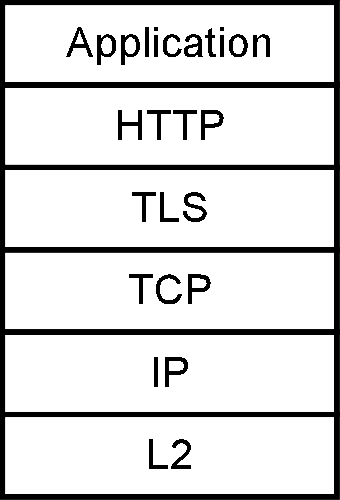
\includegraphics[width=0.25\textwidth]{5g-stack.pdf}
    \end{center}
    \caption{5G Control Plane Protocol Stack, according to TS 29.573 (\cite{3gpp.29.573}, 11)}
    \label{fig:5g-stack}
\end{wrapfigure}

\gls{3gpp} Release 15 features a redesigned protocol stack for signaling traffic between 5G core network functions, illustrated in figure \ref{fig:5g-stack}.
Rather than relying on specialized protocols that are almost exclusively used in previous generations of mobile networks, 5G makes broad use of protocols, formats, and principles popular in the domain of web services.
The \gls{tcp} is used on transport layer, rather than \gls{sctp}.
On top of that, \gls{ip} packets carry \gls{http}/2 messages that may optionally be protected by \gls{tls}.
Inside the \gls{http}/2 body additional information structured as \gls{json} objects can be transferred.
Communication between 5G core network \glspl{nf} evolves around \glspl{api} that are modelled according the principle of \gls{rest}.
This design decision brings with it a number of constrains originally layed out by \cite{fielding2000arch}.
The ones currently adopted by \gls{3gpp} for the signaling between 5G core network nodes are:\\

\begin{enumerate}[label=\arabic*)]
    \item \textit{Resources, Resource Identifiers, and Resource Representation}

    Every single data point that might be the target of a signaling message is considered a resource.
    A resource is an abstract entity that may be referenced by identifiers.
    Its information can be conveyed in varying representations, e.g. a \gls{json} object.

    \item \textit{Client-Server Communication}

    Communication follows a strict separation of concerns, allowing both client and server to evolve independently as long as the defined \glspl{api} are used.
    In the \gls{3gpp} specification the terms consuming \gls{nf} and producing \gls{nf} are equally used.

    \item \textit{Statelessness}

    Signaling messages are expected to be completely self-contained, allowing the receiving party to intepret them without any additional state information stored across multiple requests/responses.
    Although this holds true for \gls{http} itself, both \gls{tls} and \gls{prins} being stateful protocols do not adhere to this constraint.

    \item \textit{Cache}

    Resulting from item 3) is the ability of the client or intermediaries to store certain responses temporarily for future (re-)use.
    A possible way to optimize intra-\gls{plmn} signaling latency, this behaviour is not relevant for inter-operator communication.

    \item \textit{Layered Systems}

    This constraint demands that the client does not need to be aware of what exactly happens on server side to fulfill a request or even which server instance is answering.
    In essence, this is about decoupling of individual services which is inherent to the design of the 5G core network.

\end{enumerate}

The above-mentioned changes to the protocol stack also extend to the signaling channel between different \glspl{plmn}, i.e. the N32 interface.
But aside from modernizing the protocols, a redesigned Core Network architecture entails further changes to enhance interconnect security.
Whereas earlier mobile generations only specify protection on transport layer by means of IPsec, which in practice is rarely used due to operator requirements cited in the previous section, 5G aims to offer more flexible protection on application layer.
For this purpose, a dedicated Network Function is introduced to ensure security on the N32 interface.
The \gls{sepp} is tasked with applying confidentiality and integrity protection to outbound signaling messages, depending on an operator-controlled protection policy.
Simultaneously, it is the single point of contact for all inbound signaling traffic, ensuring mutual authentication with all peer \glspl{sepp}, enforcing message integrity, rate limits, and further security checks.
A complete list of \gls{sepp} requirements is given in TS 33.501 (\cite{3gpp.33.501}, 31).

When an \gls{nf} needs to exchange \gls{gls:cp} messages with an entity in a different \gls{plmn}, it addresses the \gls{sepp} in its own network.
The \gls{sepp} transforms the complete \gls{http} message into a \gls{json} object before applying security on the individual information elements contained.
Protection is provided by means of \gls{jwe} and symmetric keys shared between peer \glspl{sepp}.
Afterwards, the transformed message sent on the N32 interface towards the roaming partner's \gls{sepp} via one or more \gls{ipx} providers.
Certain \gls{ipx} providers may add changes to the transported messages, using the \gls{json} patch method specified in RFC 6902  (\cite{rfc6902}).
Each patch is digitally signed using \gls{jws} and the \gls{ipx} provider's private key.
Before any message modifications are possible, the related public key needs to be shared with the involved \glspl{mno}.
By relying on asymmetric cryptography, traceability of any intermediary patches can be ensured.
Once a \gls{sepp} receives an incoming message on N32 , it validates the integrity of the original contents and any patches added by \gls{ipx} providers.
If this first validation is successful and the added \gls{json} patches only modify information elements that are allowed to be accessed, the \gls{sepp} transforms the \gls{json} element back into a signaling message, applying changes by the \gls{ipx} providers in the process.
The resulting \gls{http} message is forwarded to the destination \gls{nf}.
This flow is illustrated in figure \ref{fig:n32} below.

\begin{figure}[h!]
    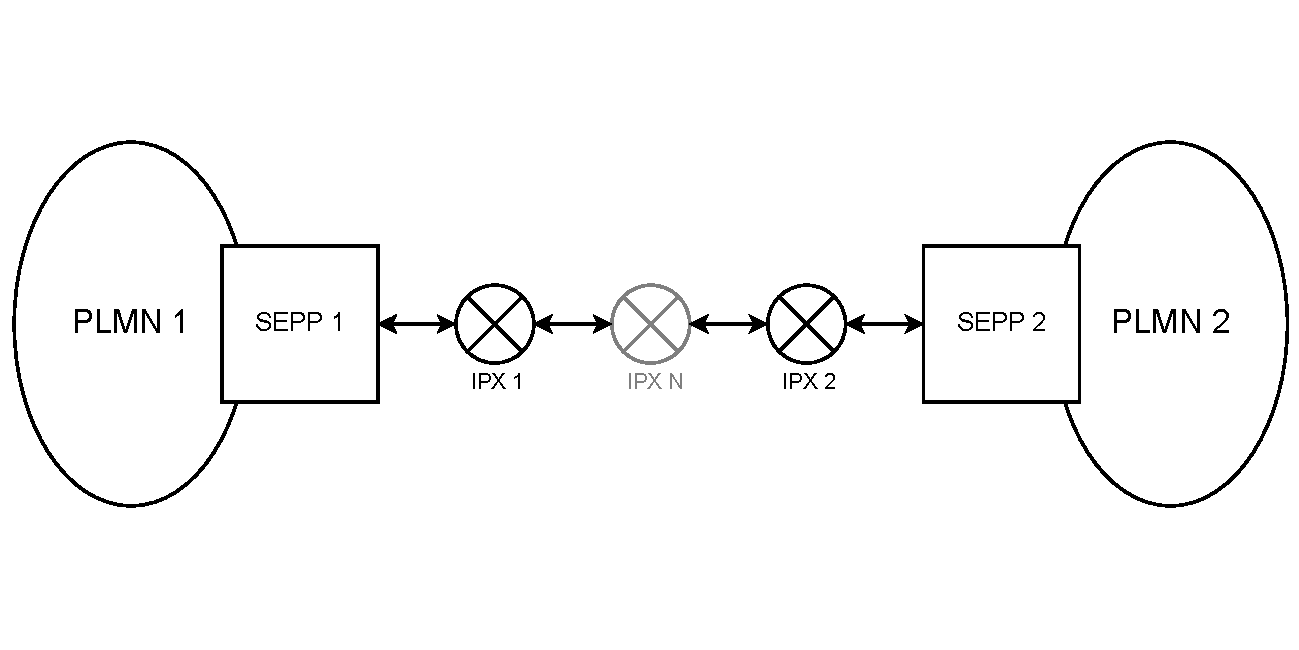
\includegraphics[width=\linewidth]{5g-roaming-arch.pdf}
    \centering
    \caption{5G interconnect architecture, according to TS 33.501 (\cite{3gpp.33.501}, 128)}
    \label{fig:n32}
\end{figure}

\subsection{The PRINS Protocol}
\subsubsection{Protocol Structure}

The 5G inter-operator signaling protocol provides security for messages on the N32 interface between two \glspl{sepp}.
It allows these two endpoints to specify the level of protection prior to establishing a connection using so-called protection policies.
The protocol is comprised of two logical channels.
\\

\textbf{N32-c} is a \gls{tls}-protected connection used for session management.
Once an interconnect session is established, each of the communicating \glspl{sepp} sets up an N32-c channel to be able to send and receive such messages by its peer.
Messages exchanged via this channel serve the purpose of session key agreement and refesh, session parameter agreement (e.g. protection policies and cryptographic profiles), and error handling throughout the session. Since none of these use cases require access to the message contents by any intermediaries, they are being carried out via a separate end-to-end protected channel.

In case two \glspl{plmn} are directly connected, without any intermediaries whatsoever, \gls{3gpp} also specifies the option to utilize the N32-c channel to transfer signaling messages directly, without the use of \gls{prins}.
This purely \gls{tls}-based operation is highlighted for completeness sake and shall not be analyzed in details, for reasons cited in section~\ref{sec:goal}.
\\

\textbf{N32-f} is a \gls{prins}-protected connection carrying \gls{http} messages that contain the inter-operator signaling data serialized as \gls{json} objects.
The level of protection provided for individual information elements on this channel is determined by two types of protection policies, specified by the communicating parties:

\begin{enumerate}[label=--]
    \item \textit{Data-type encryption policy}, describing what types of information elements require confidentiality protection.
    \item \textit{Modification policy}, describing what information elements are allowed to be modified by intermediaries \gls{ipx} providers.
\end{enumerate}

The data-type encryption policy is supported by an \textit{\gls{nf} \gls{api} data-type placement mapping}, defining the data-type of a particular information element.
It is specific per roaming partner, i.e. peer \gls{plmn}.
\gls{prins} expects this policy to be the same in both communicating \glspl{sepp} in order to rule out inconsistencies in confidentiality requirements.
The specification does not describe how such mismatch is to be be handled.
In addition to the operator-defined data-type encryption policies, \gls{3gpp} defines a set of types that are to be confidentiality protected by default, i.e. data of type ,,authentication vector'', ,,location data'', and ,,cryptographic material''.
Protection policies by the operator shall not contradict these default policies.
The specification does not describe how such mismatch is to be be handled.

The modification policy defined by each communicating party is only applicable to the \gls{ipx} provider that the defining \gls{mno} has a business relationship with, i.e. any mobile network operator can only actively allow changes by its directly connected interconnection providers.
By default, modifications are prohibited.
The policy is specific per roaming partner, i.e. peer \gls{plmn}, and per \gls{ipx} provider.

An N32-f session is identified by an \textit{N32-f context} -- supplementary session information stored by each \gls{sepp} in order to correlate and validate different messages.
This information can be summarized as follows:

\begin{enumerate}[label=--]
    \item \textit{N32-f context ID}, uniquely identifying a given N32-f session.
    \item \textit{N32-f peer information}, containing the peer \gls{plmn} ID, peer \gls{sepp} ID, and its \gls{ip} address.
    \item \textit{N32-f security context}, incl. the \gls{prins} session keys, \gls{jose} cipher suites, protection policies, session counters, initialization vectors, and a so-called \gls{ipx} security information list.
    \item \textit{N32-f context information}, containing details on session validity and an indication whether to use \gls{prins} or \gls{tls}.
\end{enumerate}

The N32-f context ID is created by both \glspl{sepp} during the initial handshake procedure described in the following subsection.
It is referenced in each N32-f message in order to inform the receiving \gls{sepp} which session to correlate it to.

The N32-f peer information holds the \gls{plmn} ID and an additional \gls{sepp} ID in order to differentiate multiple instances in the foreign network.
A remote \gls{sepp} address is required for routing purposes.

The security context contains the complete N32-f key hierarchy, which is comprised of a single master key generated from the initial N32-c \gls{tls} session, using the \gls{tls} export mechanism specified in RFC 5705 (\cite{rfc5705}), as well as two sets of session keys and \gls{iv} derived form the master key and sequence counters.
The latter are used for applying \gls{jwe} protection to N32-f messages -- keys for encryption, \glspl{iv} and counters for constructing the nonce required by \gls{aes}-\gls{gcm}.
Two sets of each are required since N32-f, similar to N32-c, requires setting up two distinct \gls{http} connections to enable a \gls{sepp} to both send and receive messages.
Hence, \gls{3gpp} specifies ,,parallel'' session keys and \glspl{iv} for use by the \gls{sepp} that initialted the N32-c session.
The other sets of ,,reverse'' session keys and \glspl{iv} are to be used for a \gls{prins} session with the \gls{sepp} that responded to the initial N32-c establishment.

\begin{minipage}[l]{0.5\textwidth}
    \begin{enumerate}[label=--]
        \item \texttt{parallel\_request\_key}
        \item \texttt{parallel\_response\_key}
        \item \texttt{parallel\_request\_iv\_salt}
        \item \texttt{parallel\_response\_iv\_salt}
    \end{enumerate}
\end{minipage}%
\begin{minipage}[r]{0.5\textwidth}
    \begin{enumerate}[label=--]
        \item \texttt{reverse\_request\_key}
        \item \texttt{reverse\_response\_key}
        \item \texttt{reverse\_request\_iv\_salt}
        \item \texttt{reverse\_response\_iv\_salt}
    \end{enumerate}
\end{minipage}\\

Furthermore, the aforementioned protection policies are referenced in the N32-f context, as their intended scope is a particular N32-f session.
The agreed cryptographic algorithms for \gls{jwe} protection are stored as cipher suites.
Lastly, the N32-f security context holds an \gls{ipx} security information list -- identifiers of all intermediary \gls{ipx} providers as well as dedicated raw public keys or certificates used to validate message modifications sumbitted by them.

\subsubsection{PRINS Message Format}

Signaling messages sent towards receivers in a different \gls{plmn} are reformatted into a \gls{json} structure by the \gls{sepp} before being forwarded on the N32 interface.
Depending on the protection requirements described in the configured policies, individual parts of the original \gls{http} message are placed in different locations.
\gls{3gpp} defines two objects to be created by the sending \gls{sepp}.
An example message is provided in figure XYZ.

\begin{enumerate}[label=--]
    \item \textit{dataToIntegrityProtect} holds all information to be integrity protected.
    This includes the complete messages with all its pseudo-header fields (e.g. \gls{http} method), \gls{http} headers, and the \gls{http} body with the exception of information elements requiring confidentiality protection, whose values are replaced by null.
    The \gls{sepp} further supplies additional N32-f specific meta data, i.e. N32-f message ID, N32-f context ID, and an ID of the directly connected \gls{ipx} provider.

    \item \textit{dataToIntegrityProtectAndCipher} contains information to be both integrity and confidentiality protected.
    The \gls{sepp} creates a \gls{json} patch for each of the concerned elements of the original message and such that there is a patch replacing each of the null values in the dataToIntegrityProtect object.
\end{enumerate}

Following the reformatting, both of these \gls{json} objects are protected using \gls{jwe}.
For this purpose, \gls{3gpp} only specifies encryption methods that build on \gls{aead}, i.e. cryptographic schemes ensuring both confidentiality and authenticity of data.
The use of \gls{jwe} with these particular cipher suites allows for the choice to protect integrity and confidentiality of certain objects while others are only integrity protected, depending how they are fed into the \gls{aead} algorithm:
The dataToIntegrityProtectAndCipher object serves as input for the encryption whereas the dataToIntegrityProtect object is used as \gls{aad}.
Resulting from this operation is the ciphertext itself and a \gls{jwe} Authentication Tag, which can be used to verify the integrity of both the ciphertext and \gls{aad}.

\subsubsection{Protocol Sequences}
